\documentclass{article}
\usepackage[utf8]{inputenc}
\usepackage{authblk}
\usepackage{setspace}
\usepackage[margin=1.25in]{geometry}
\usepackage{graphicx}
\usepackage{xcolor}
\usepackage{float}
\graphicspath{ {./figures/} }
\usepackage{amsmath,amssymb,amsfonts}
\usepackage{booktabs}
\usepackage{natbib}
\usepackage{hyperref}
\hypersetup{colorlinks=true, linkcolor=blue, citecolor=blue, urlcolor=blue}

\title{\textbf{The Turn-of-the-Month Effect in the US Stock Index, 2016--2026}}
\author[1]{SIQuant Research}
\affil[1]{Hypothesis $\times$ Quant}
\date{\today}
\onehalfspacing

\begin{document}
\maketitle

\begin{abstract}
\noindent \textbf{Hypothesis:} $H_0$: the mean daily S\&P 500 return on turn-of-month sessions equals that of other sessions; $H_1$: it is larger \\
\textbf{Data:} 2,491 sessions, 2016-11-01 to 2026-09-30; 476 turn-of-month sessions (19.1\% of days) \\
\textbf{Method:} Last session of the month plus the first three of the next; 10,000-draw placebo over other sessions \\
\textbf{Results:} Mean 0.069\% versus placebo 0.055\% (one-sided $p=0.3904$); the window carries 23\% of the cumulative log-return sum. \\
\textbf{Research decision:} \colorbox[rgb]{0.75,0.15,0.15}{\textcolor{white}{\textbf{\,REJECTED\,}}}
\end{abstract}

\section{Design}
The window is the classic one of \citet{lakonishok1988turn}, fixed in advance. The first and last month of the data are dropped because their edges are incomplete. The placebo draws the same number of sessions from outside the window, which keeps the volatility regime matched on average.

\section{Results}
\begin{table}[H]
\centering
\caption{Mean daily S\&P 500 return by year}
\begin{tabular}{lcc}
\toprule
Year & Turn-of-month & Other sessions \\
\midrule
2016 & -0.279\% & 0.220\% \\
2017 & 0.087\% & 0.068\% \\
2018 & -0.023\% & -0.019\% \\
2019 & 0.068\% & 0.112\% \\
2020 & 0.321\% & 0.028\% \\
2021 & 0.036\% & 0.113\% \\
2022 & -0.049\% & -0.081\% \\
2023 & 0.137\% & 0.079\% \\
2024 & -0.098\% & 0.130\% \\
2025 & 0.032\% & 0.076\% \\
2026 & 0.299\% & 0.007\% \\
\bottomrule
\end{tabular}
\end{table}


\begin{figure}[H]
\centering
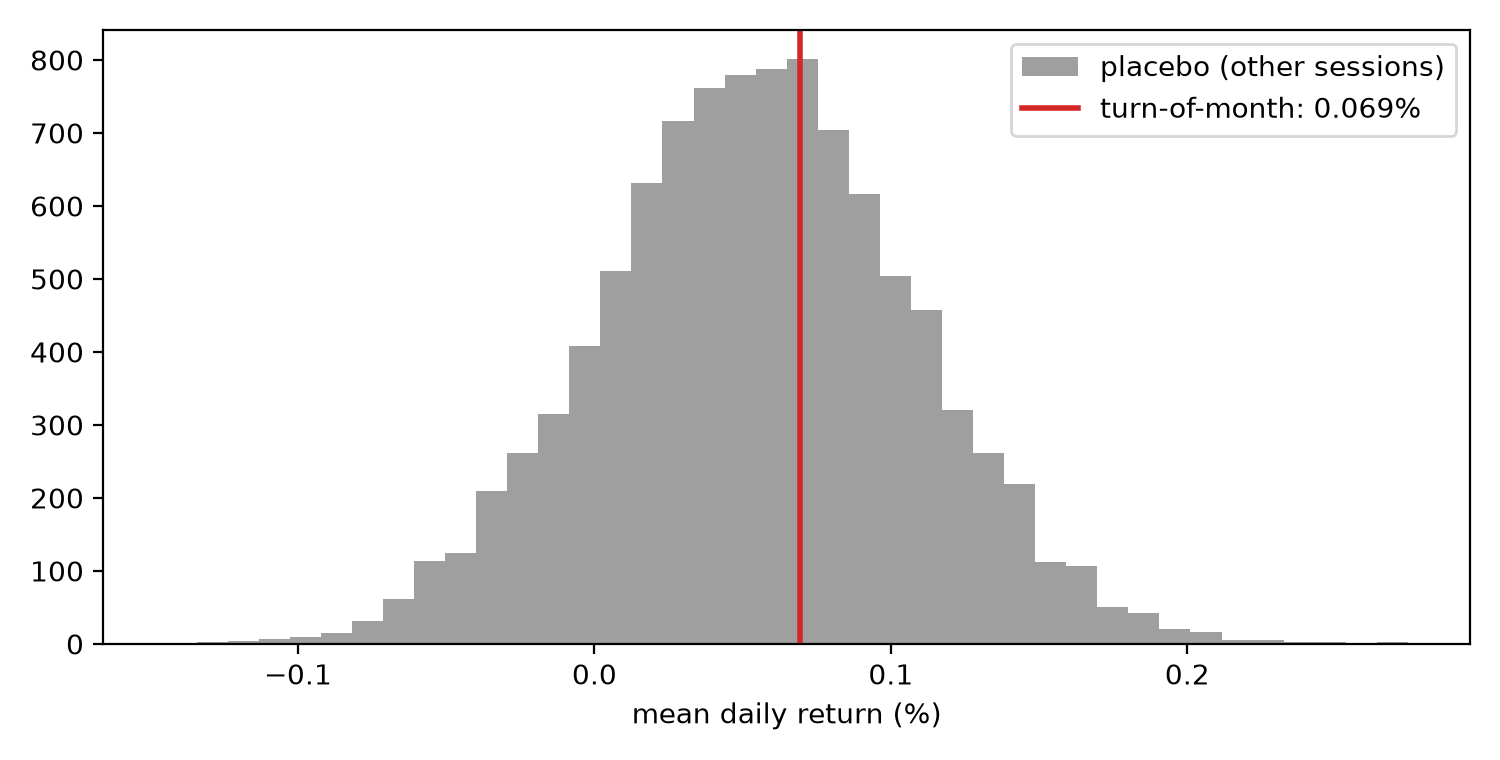
\includegraphics[width=0.8\textwidth]{fig1_tom_placebo.png}
\caption{Turn-of-month mean return against the placebo distribution.}
\end{figure}

\section{Limitations}
A calendar effect documented in the literature may be arbitraged away; ten years contain about 120 windows. Placebo draws ignore serial dependence, which is small for daily index returns.


\bibliographystyle{plainnat}
\bibliography{references}

\end{document}
